%!TEX root = ../thesis.tex

本章では, 従来研究を基にしたオフラインでデータを収集し訓練する手法を提案する.

\section{手法}
本研究で検証するオフライン手法に関して述べる. オンライン手法と比べて, オフライン手法は画像と目標角速度のデータを事前に収集して, 学習するところが異なる. \figref{Fig:collect-data2}にシミュレータを用いて収集するデータを示す. 目標経路(赤線)から一定距離の位置にロボットを配置して, さらに目標経路の方向を基準として, ヨー方向に一定量回転する. その時の中央のカメラの画像と, 目標角速度を収集してデータセットに加える. ちなみに, 本手法でデータを収集するためには, 非常に多くのロボットの置き直しをしなければならない. これを, 実ロボットに応用する際には, 1台のロボットに複数のカメラを搭載して, 経路から一定距離離れた画像を収集する. そうすることで, 置き直ししなくても経路を走行すればデータを集められる. そのため,実ロボットへの応用も可能であると考える. このように収集したデータセットを用いてオフラインで学習する. なお,リアルタイム性に配慮して, オンライン手法ではバッチサイズ8のミニバッチ学習を行っていたが, オフライン学習ではリアルタイム性は必要ないため, バッチ学習を行う. 

% \vspace{10mm}
\newpage
  \begin{figure}[h]
  \centering
  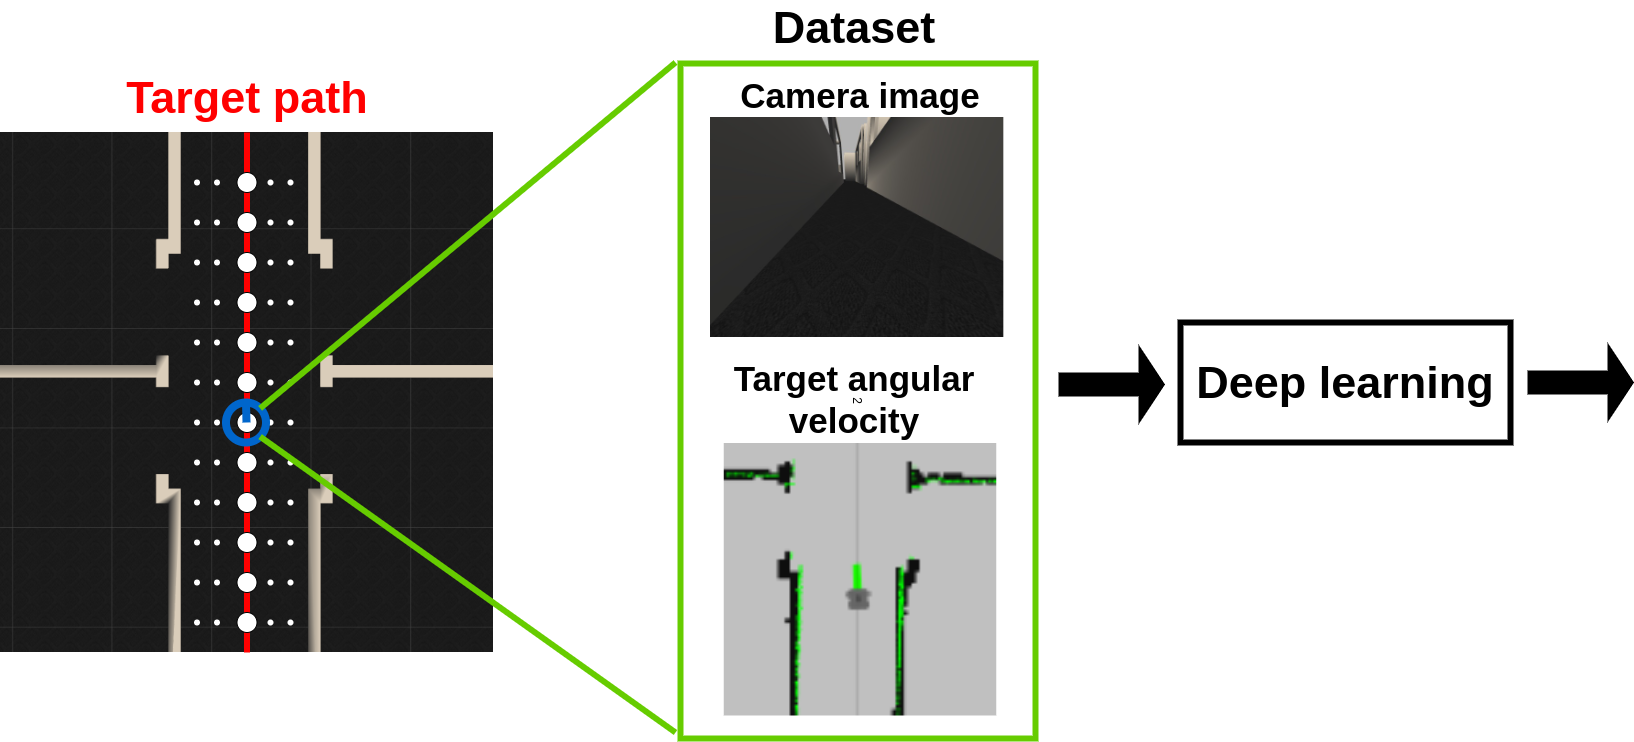
\includegraphics[keepaspectratio, scale=0.2]{images/collect-data2.png}
  \caption{Data collected by the simulator in the learning phase}
  \label{Fig:collect-data2}
  \end{figure}

